\chapter{Vision Transformers (ViT)}

\section{Why CNNs Are Not Enough}

Since the introduction of AlexNet in 2012, CNNs have been the dominant architecture for computer vision. Despite their success, CNNs possess inherent architectural limitations. Their reliance on local convolutional operations makes modeling long-range dependencies difficult and often requires increasingly deep networks to capture global context.

These limitations motivated researchers to investigate whether the Transformer architecture, which had already revolutionized Natural Language Processing, could also replace CNNs in computer vision.

Many visual recognition tasks require understanding interactions between objects that are spatially far apart. A local convolution cannot directly relate two distant image regions; instead, information must propagate gradually through multiple convolution layers. Consequently, capturing global context becomes increasingly difficult as image size grows.

\subsection{Motivation for Vision Transformers (ViT)}

The Vision Transformer was designed around a simple question:
\begin{center}
\textbf{Can an image be treated like a sentence?}
\end{center}

The key insight behind ViT was that an image can also be represented as a sequence by dividing it into small patches.

Once converted into a sequence of patches, the standard Transformer encoder can process the image without using any convolutional layers. This idea became the foundation of modern Vision Transformers.

\subsubsection*{Advantages}
\begin{itemize}
    \item Direct modeling of long-range dependencies.
    \item Global receptive field from the first attention layer.
    \item Greater flexibility with larger datasets and models.
    \item Better scalability due to weaker inductive bias.
    \item Unified architecture for both language and vision.
\end{itemize}

However, these benefits come at the cost of increasing data requirements and higher computational complexity, motivating later improvements such as DeiT, Swin Transformer, and Masked Autoencoders.


\section{Image to Sequence}

The key idea of the ViT is to divide the image into fixed-size patches and treat each patch as a token, just as words are treated as tokens in NLP.

Instead of processing individual pixels, ViT divides the image into non-overlapping square patches.
\begin{figure}[H]
\centering
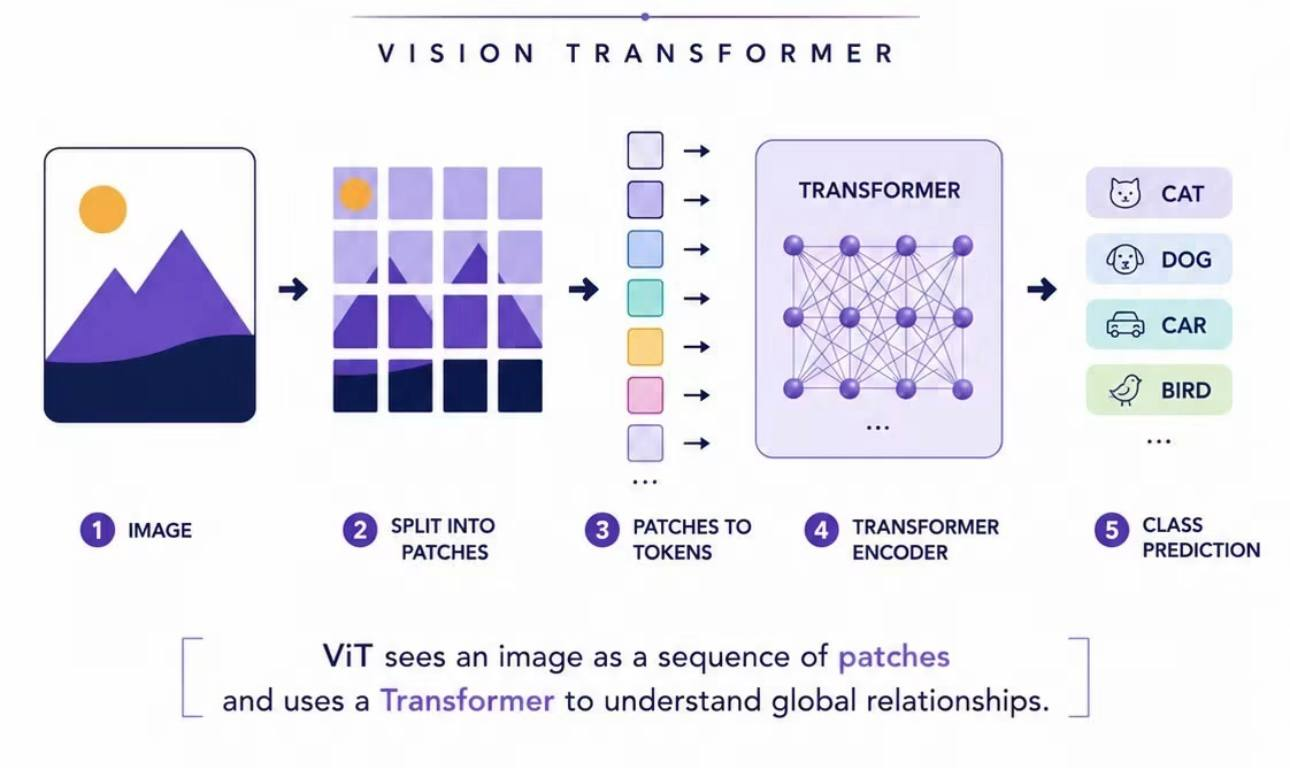
\includegraphics[width=0.95\textwidth]{figures/vit patches.jpg}
\end{figure}
\begin{itemize}
    \item \textbf{Image Size}: $224 \times 224 \times 3$
    \item \textbf{Patch Size}: $16 \times 16$: The image is divided into small $16 \times 16$ RGB patches.
\end{itemize}

\subsection{Number of Patches}
\[
N = \frac{H}{P} \times \frac{W}{P} \implies N = \frac{224}{16} \times \frac{224}{16} = 14 \times 14 = 196
\]

\subsection{Flattening Each Patch}
Each patch still has three dimensions ($16 \times 16 \times 3$). Before being processed by the Transformer, each patch is flattened into a one-dimensional vector:
\[
16 \times 16 \times 3 = 768
\]
Every patch is now represented by a vector containing 768 values.

After flattening all patches, the original image is transformed into a sequence. The resulting tensor is $196 \times 768$. Instead of a 2D image, the Transformer now receives a sequence of 196 vectors.


\section{Patch Embedding}

After dividing the image into patches, each patch is represented as a flattened vector. However, these vectors cannot be fed directly into the Transformer because the Transformer expects every input token to have the same embedding dimension $d_{\text{model}}$.

Therefore, each flattened patch is projected to a fixed-dimension embedding space using a learnable linear layer. This process is called \textbf{Patch Embedding}.

The Transformer expects embeddings of dimension $d_{\text{model}}$, for example:
\begin{itemize}
    \item \textbf{ViT-Base}: $d_{\text{model}} = 768$
    \item \textbf{ViT-Large}: $d_{\text{model}} = 1024$
    \item \textbf{ViT-Huge}: $d_{\text{model}} = 1280$
\end{itemize}

Therefore, every patch must be transformed into a vector of size $d_{\text{model}}$.


\section{Positional Embedding}

After patch embedding, Vision Transformers add learnable positional embeddings to preserve the spatial arrangement of image patches.

Unlike the original Transformer (2017) which used fixed sinusoidal positional encodings, ViT uses learnable positional embeddings:
\[
E_{\text{pos}} \in \mathbb{R}^{(N+1) \times d_{\text{model}}}
\]
\begin{itemize}
    \item $N =$ Number of image patches
    \item $+1 =$ The CLS token
    \item $d_{\text{model}} =$ Embedding dimension
\end{itemize}

Each position has its own learnable vector. These vectors are initialized randomly and optimized during training.

\subsection{Adding Positional Embeddings}
\[
X = E_{\text{patch}} + E_{\text{pos}}
\]
Each patch embedding now contains:
\begin{itemize}
    \item Visual information.
    \item Spatial position.
\end{itemize}

\subsection{Why Add the CLS Token First?}

The CLS token is treated like an additional patch. Therefore, it also requires positional information. For this reason, the CLS token is first appended to the patch sequence, and then positional embeddings are added to all tokens simultaneously. This ensures that the CLS token has its own learnable positional embedding.


\section{CLS Token}

Unlike NLP, where the output may consist of multiple tokens, image classification requires only one prediction for the entire image.

The Vision Transformer solves this problem by introducing a special learnable token called the \textbf{CLS (Classification) Token}.

Instead of representing a single image patch, the CLS token is designed to collect information from all image patches through self-attention. After passing through all Transformer encoder layers, it serves as a compact representation of the entire image and is used for classification.

Before entering the Transformer encoder, a learnable CLS token is prepended to the sequence of patch embeddings:
\[
\text{If patch embeddings are } [P_1, P_2, \dots, P_N]
\]
\[
\text{The input sequence becomes } [\text{CLS}, P_1, P_2, \dots, P_N]
\]
\[
196 \times 768 \longrightarrow 197 \times 768
\]
\[
\text{CLS} \in \mathbb{R}^{d_{\text{model}}}
\]

Initially, it contains random values, but during training it learns how to gather the most useful information for the target task.

During every attention layer:
\begin{itemize}
    \item The CLS token attends to every image patch.
    \item Every image patch can also attend to the CLS token.
\end{itemize}

By the end of the encoder, the CLS token becomes a global representation of the image.


\section{Classification Head}

After the final encoder layer, only the CLS token is used for image classification.

The CLS embedding is passed through a linear classification head:
\[
y = \text{CLS} \cdot W + b
\]
The resulting logits are converted into class probabilities using Softmax.

The CLS token provides several advantages:
\begin{itemize}
    \item Produces a single representation for the entire image.
    \item Learns which regions are most important through attention.
    \item Keeps the architecture simple.
    \item Can be reused for downstream tasks after fine-tuning.
\end{itemize}

\section{Vision Transformer (ViT) Architecture}

Vision Transformer (ViT), proposed by Google Research in 2020, was the first architecture to successfully apply the standard Transformer encoder directly to image classification.

Unlike CNNs, which rely on convolutional layers to extract features, ViT processes an image as a sequence of patches and uses only Transformer encoder blocks to learn visual representations. The central idea is simple: \textbf{An image can be treated like a sentence, where each image patch is equivalent to a word (token).}

\begin{figure}[H]
    \centering
    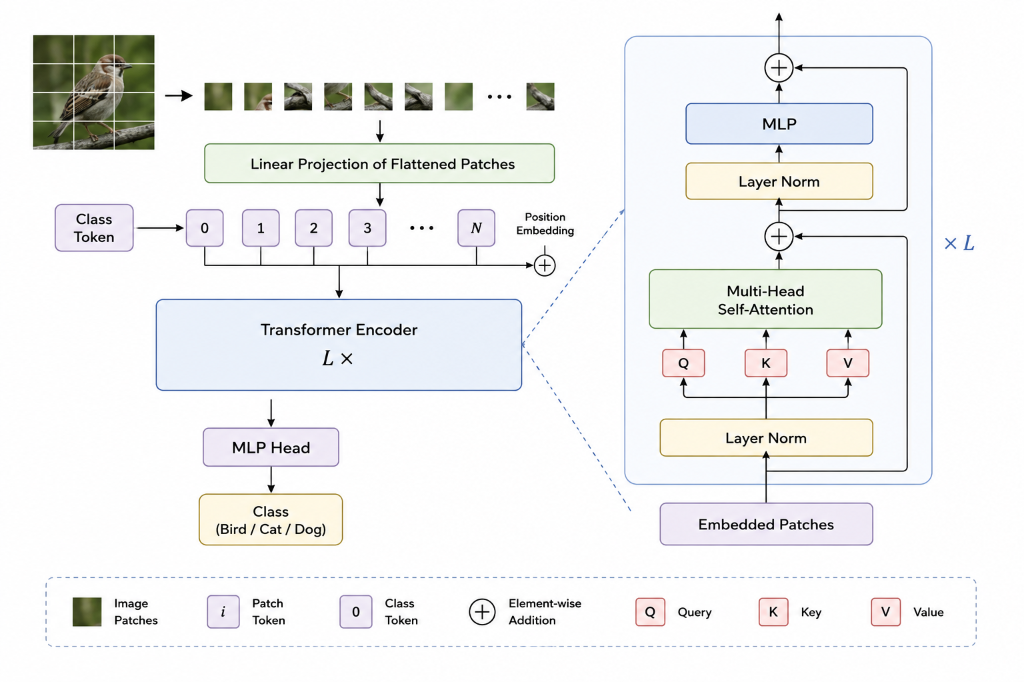
\includegraphics[width=0.92\linewidth]{figures/fig_6_vit.png}
    \caption{Vision Transformer (ViT) Architecture.}
    \label{fig:vit_architecture}
\end{figure}



The most common Vision Transformers are:
\begin{center}
\begin{tabular}{lcc}
\hline
\textbf{Model} & \textbf{Encoder Blocks} & \textbf{Parameters} \\
\hline
ViT-Base & 12 & 86 M \\
ViT-Large & 24 & 307 M \\
ViT-Huge & 32 & 632 M \\
\hline
\end{tabular}
\end{center}

\subsection{Limitations of ViT}
\begin{itemize}
    \item Requires very large training datasets.
    \item Higher computational cost than CNNs.
    \item Quadratic attention complexity ($\mathcal{O}(N^2)$).
    \item Less data-efficient because it lacks CNN inductive bias.
\end{itemize}

These limitations motivated several improved architectures including:
\begin{itemize}
    \item \textbf{DeiT}: More data-efficient training.
    \item \textbf{Swin Transformer}: Linear attention complexity.
    \item \textbf{MAE}: Self-supervised pretraining.
\end{itemize}

Vision Transformers have very weak inductive biases. They must learn spatial relationships directly from data, which requires much larger datasets and more computational resources. The original ViT paper demonstrated that training directly on ImageNet-1K (1.3 million images) was not sufficient to outperform state-of-the-art CNNs.

Instead, pretrained ViT on much larger datasets before fine-tuning on ImageNet. The largest datasets used included:
\begin{itemize}
    \item \textbf{ImageNet-21K}: $\sim 14$ million images, 21,000 classes.
    \item \textbf{JFT-300M}: $\sim 300$ million images, proprietary Google dataset.
\end{itemize}

Pretraining on these massive datasets allowed ViT to learn rich visual representations.

After large-scale pretraining, the model is adapted to a specific downstream task through fine-tuning. Typically, only the final classification layer is replaced to match the number of classes in the new dataset, while the pretrained encoder weights are reused and further optimized.


\section{DeiT (Data-efficient Image Transformer)}

One of the biggest criticisms of the original Vision Transformer was that it required hundreds of millions of training images to outperform CNNs. This made ViT impractical for most researchers and companies.

In 2021, Facebook AI introduced DeiT, demonstrating that Vision Transformers could be trained using only ImageNet while achieving competitive performance. The key innovation was \textbf{Knowledge Distillation} adapted specifically for Vision Transformers.

\subsection{The Problem with ViT}
\begin{itemize}
    \item Very large datasets.
    \item Extremely long training.
    \item Huge computational resources.
\end{itemize}

Without massive pretraining, CNNs like ResNet generally performed better. The challenge was therefore: \textbf{Can a Vision Transformer learn efficiently from a relatively small dataset?} DeiT answered \textbf{yes}.

\subsection{Main Contributions of DeiT}

DeiT introduced three major improvements:
\begin{enumerate}
    \item Efficient training recipe.
    \item Strong data augmentation and regularization.
    \item Knowledge distillation using a Distillation Token.
\end{enumerate}

\subsection{Knowledge Distillation}

Knowledge distillation is a technique where a large pretrained model (\textbf{Teacher}) transfers knowledge to a smaller model (\textbf{Student}). Instead of learning only from the ground-truth labels, the student also learns from the predictions of the teacher.

CNNs already learn excellent visual features from relatively small datasets. Instead of discarding decades of CNN research, DeiT leverages CNN knowledge to train the Transformer more effectively.

\subsection{Distillation Token}

DeiT adds another learnable token:
\[
[\text{CLS}, \text{DIST}, P_1, P_2, \dots, P_N]
\]

The input sequence now contains:
\begin{itemize}
    \item CLS Token
    \item DIST Token
    \item Image patches
\end{itemize}

During self-attention, the distillation token interacts with all image patches, just like the CLS token. However, instead of learning from the ground-truth labels, it learns to mimic the teacher model's prediction.

Thus:
\begin{itemize}
    \item \textbf{CLS Token} $\rightarrow$ Supervised by true labels.
    \item \textbf{DIST Token} $\rightarrow$ Supervised by teacher network.
\end{itemize}

The Transformer therefore learns from both supervision signals simultaneously.

\begin{figure}[H]
    \centering
    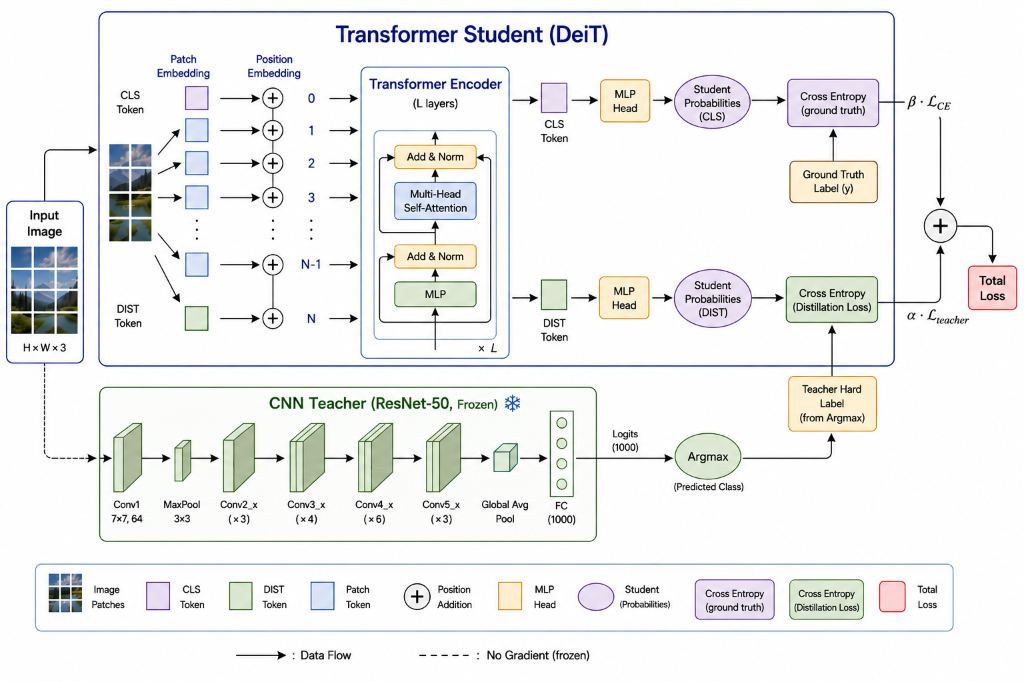
\includegraphics[width=0.92\linewidth]{figures/fig_6_deit.png}
    \caption{Transformer Student (DeiT) \& CNN Teacher (ResNet-50) Knowledge Distillation Architecture.}
    \label{fig:deit_architecture}
\end{figure}

\subsection{Inference}

After training, the teacher network is discarded. Only the DeiT model is used for inference. The teacher is needed only during training.

\subsection{Advantages (Compared to ViT)}
\begin{itemize}
    \item Much smaller training datasets.
    \item Faster convergence.
    \item Better data efficiency.
    \item Competitive performance on ImageNet-1K.
    \item No need for massive proprietary datasets.
\end{itemize}


\section{Swin Transformer (Shifted Window Transformer)}

Although the original Vision Transformer (ViT) achieved excellent accuracy, it had a major limitation: Self-attention has quadratic complexity $\mathcal{O}(N^2)$, where $N$ is the number of image patches.

As image resolution increases, the number of patches increases, making computation and memory requirements extremely expensive.

To solve this problem, Microsoft introduced the Swin Transformer in 2021. Its two main innovations are:
\begin{itemize}
    \item \textbf{Window-based Multi-head Self-Attention (W-MSA)}
    \item \textbf{Shifted Window Multi-head Self-Attention (SW-MSA)}
\end{itemize}

These ideas greatly reduce computation while still allowing information to flow across the entire image.

\subsection{Window Attention (W-MSA)}

Instead of allowing every patch to attend to every other patch, Swin divides the image into small non-overlapping windows.

\begin{figure}[H]
    \centering
    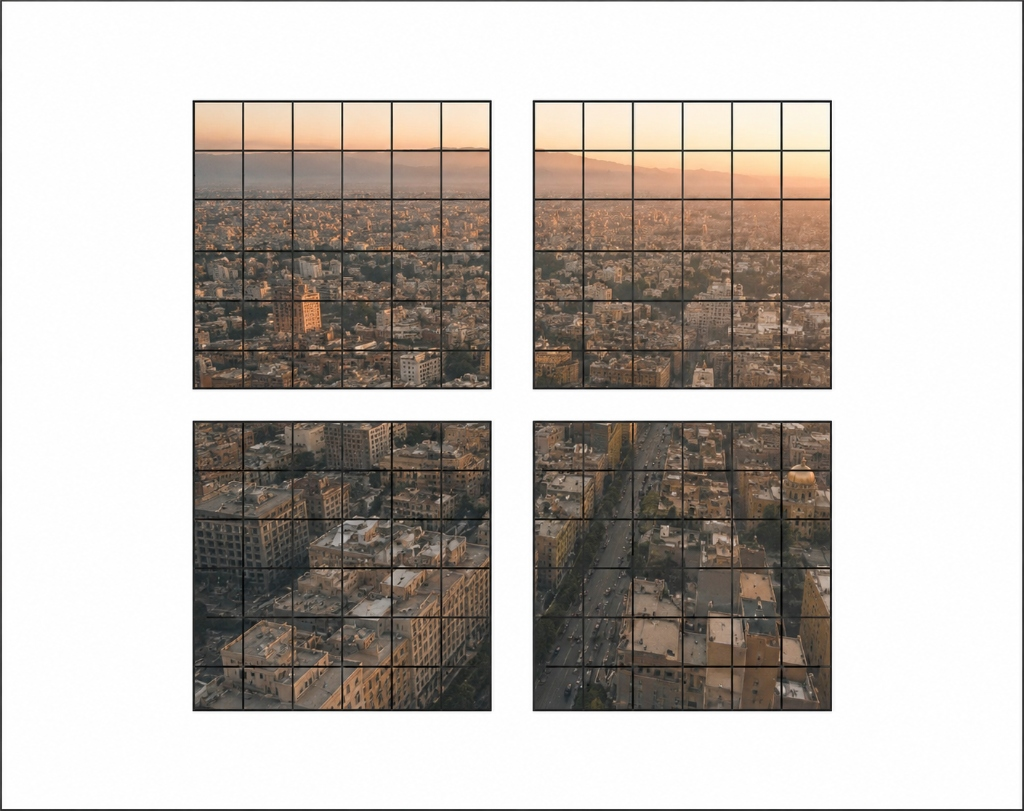
\includegraphics[width=0.75\linewidth]{figures/fig_6_swin_window_partition.jpg}
    \caption{Window Partitioning in Swin Transformer (W-MSA).}
    \label{fig:swin_window_partition}
\end{figure}

Each square window is processed independently. Inside one window, every patch attends only to patches within the same window. No attention is computed between different windows.

\subsubsection*{Computational Advantage}
Suppose Total patches $= 196$, window size $= 7 \times 7$ patches. Each window contains 49 patches. Instead of computing $196 \times 196$, each attention matrix becomes $49 \times 49$. This dramatically reduces computation. Instead of one huge attention matrix, the model computes several much smaller attention matrices.

However, it introduces a new issue:
\begin{center}
\textbf{Problem: Neighboring patches in different windows cannot communicate.}
\end{center}

\subsection{Shifted Window Attention (SW-MSA)}

This is Swin Transformer's key innovation. Instead of keeping the same window in every layer, the windows are shifted before the next attention operation.

\begin{figure}[H]
    \centering
    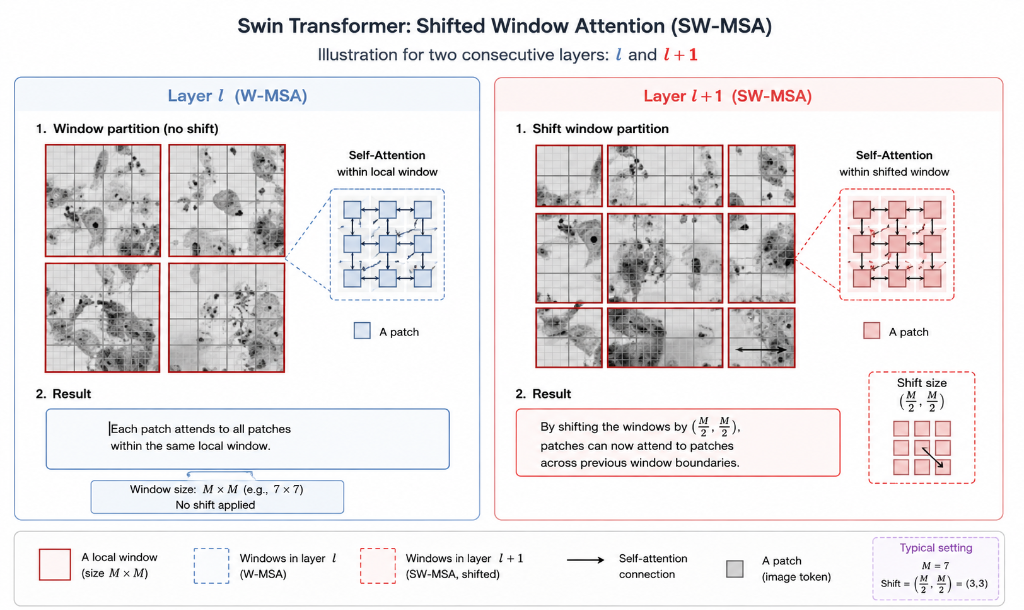
\includegraphics[width=0.90\linewidth]{figures/fig_6_swin_swmsa.png}
    \caption{Swin Transformer: Shifted Window Attention (SW-MSA) Mechanism.}
    \label{fig:swin_swmsa}
\end{figure}

The windows move by approximately half the window size (if a window contains 4 patches, so $\frac{4}{2} = 2$, it moved by 2 patches).

Patches that were previously in different windows now become part of the same window. This allows information to propagate across the entire image over multiple layers.

The process alternates between:
\begin{itemize}
    \item Window Attention (W-MSA)
    \item Shifted Window Attention (SW-MSA)
\end{itemize}

After several layers, information gradually flows across neighboring windows until the model effectively captures global context. Thus, Swin achieves a balance between:
\begin{itemize}
    \item Local efficiency.
    \item Global information exchange.
\end{itemize}




\section{Swin Architecture}

\begin{figure}[H]
    \centering
    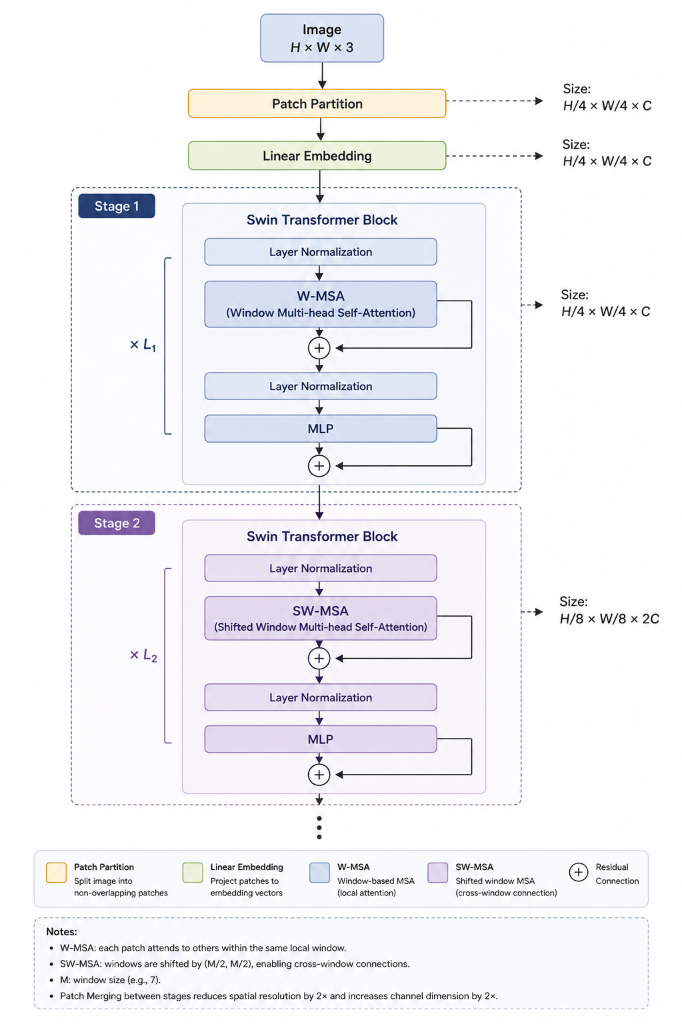
\includegraphics[width=0.88\linewidth]{figures/fig_6_swin_architecture.png}
    \caption{Swin Transformer Overall Architecture.}
    \label{fig:swin_architecture}
\end{figure}

\subsection{Two Successive Swin Transformer Blocks}

Each Stage contains Swin Transformer Blocks, and each Swin Transformer Block contains two successive Swin Transformer units (Block $l$ with W-MSA and Block $l+1$ with SW-MSA).



\begin{figure}[H]
    \centering
    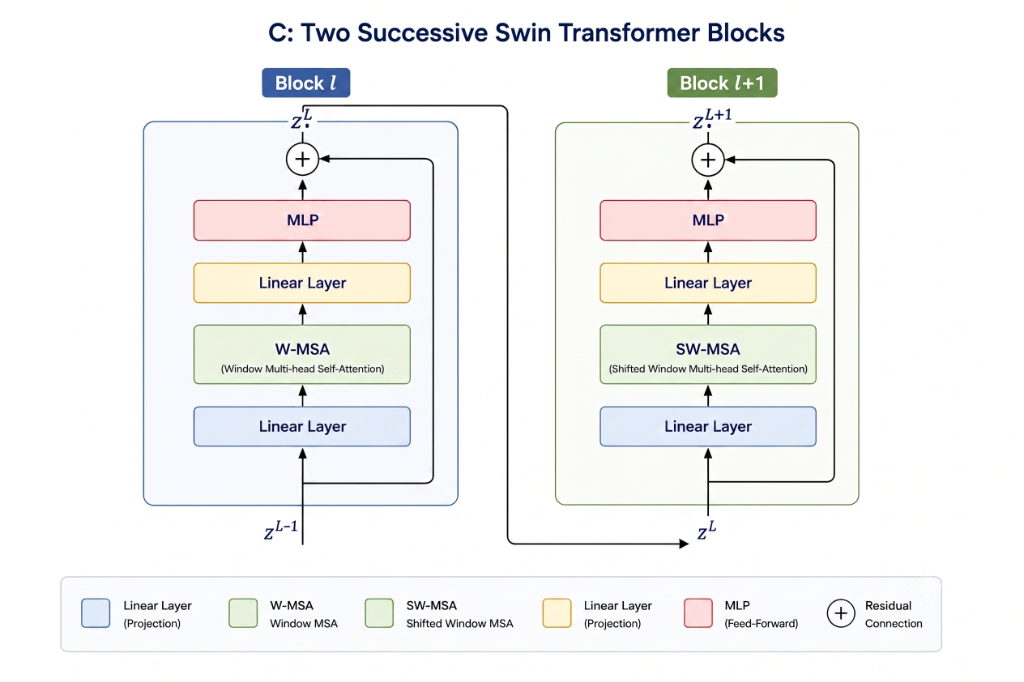
\includegraphics[width=0.82\linewidth]{figures/fig_6_swin_blocks.png}
    \caption{Two Successive Swin Transformer Blocks.}
    \label{fig:swin_blocks}
\end{figure}


\section{Summary}

\begin{itemize}
    \item The original ViT proved that Transformers could replace CNNs for image classification, but it remained computationally expensive for many vision tasks.
    \item Swin Transformer addressed this limitation by introducing window attention, shifted windows, and patch merging, making Transformers both efficient and scalable. These innovations allowed Swin to become one of the most widely adopted Transformer backbones in computer vision.
\end{itemize}
